% figures/latex_includes.tex —— 由 figures/gen_latex_includes.py 生成
% 需要 \usepackage{graphicx} 与 \usepackage{float}（[H] 就地固定，防多图堆叠）
% caption 只写短标题；口径/结论/数据来源写进正文。

\begin{figure}[H]
  \centering
  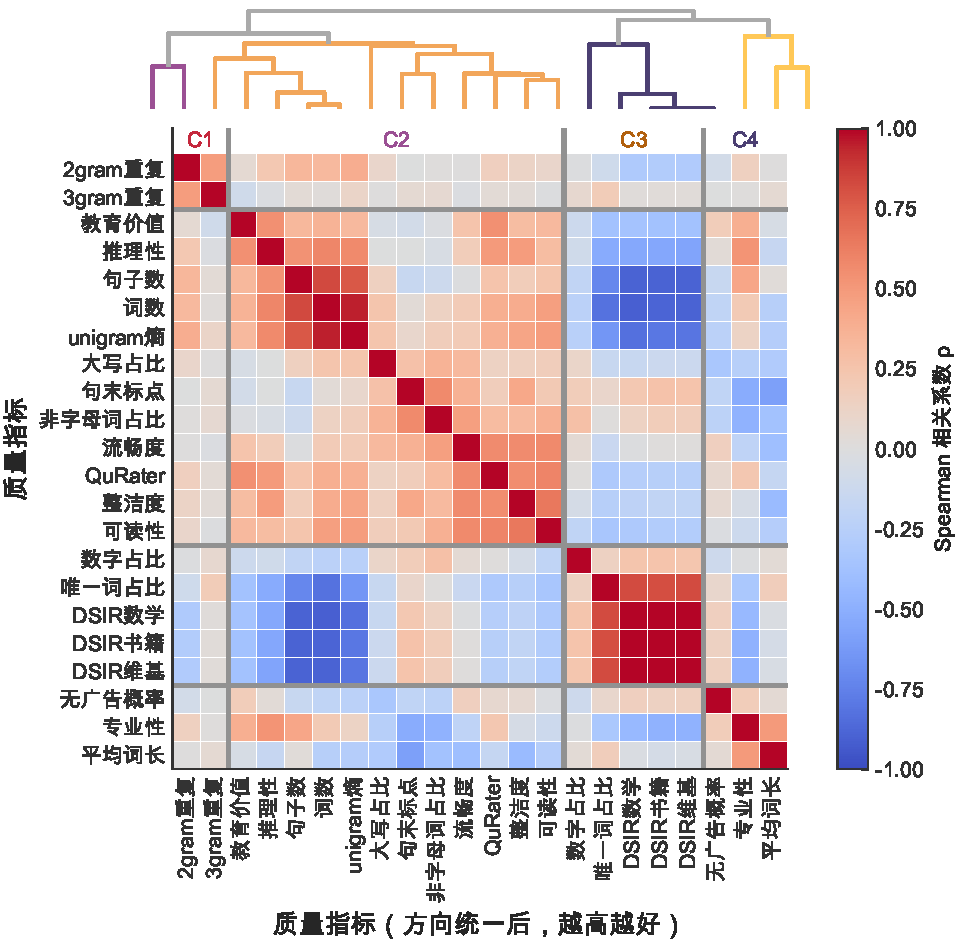
\includegraphics[width=0.8\textwidth,height=0.8\textheight,keepaspectratio]{figures/fig_q1_quality_corr.pdf}
  \caption{质量指标相关性聚类热力图}
  \label{fig:q1_quality_corr}
\end{figure}

\begin{figure}[H]
  \centering
  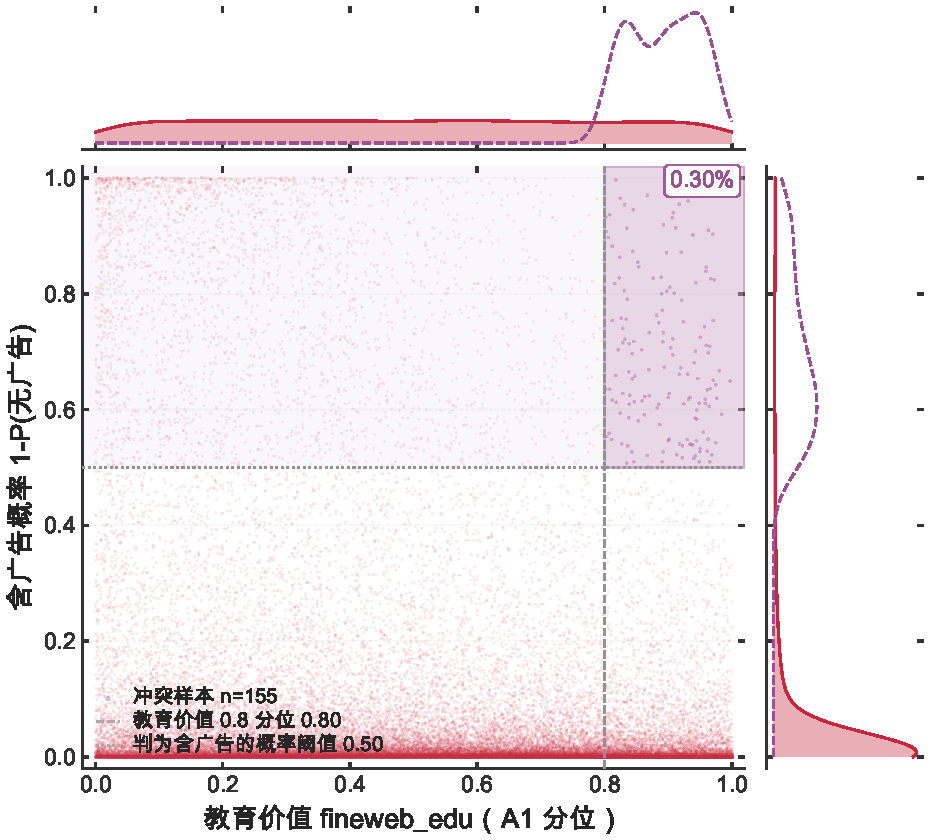
\includegraphics[width=0.8\textwidth,height=0.8\textheight,keepaspectratio]{figures/fig_q1_conflict_scatter.pdf}
  \caption{教育价值与广告含量的冲突区}
  \label{fig:q1_conflict_scatter}
\end{figure}

\begin{figure}[H]
  \centering
  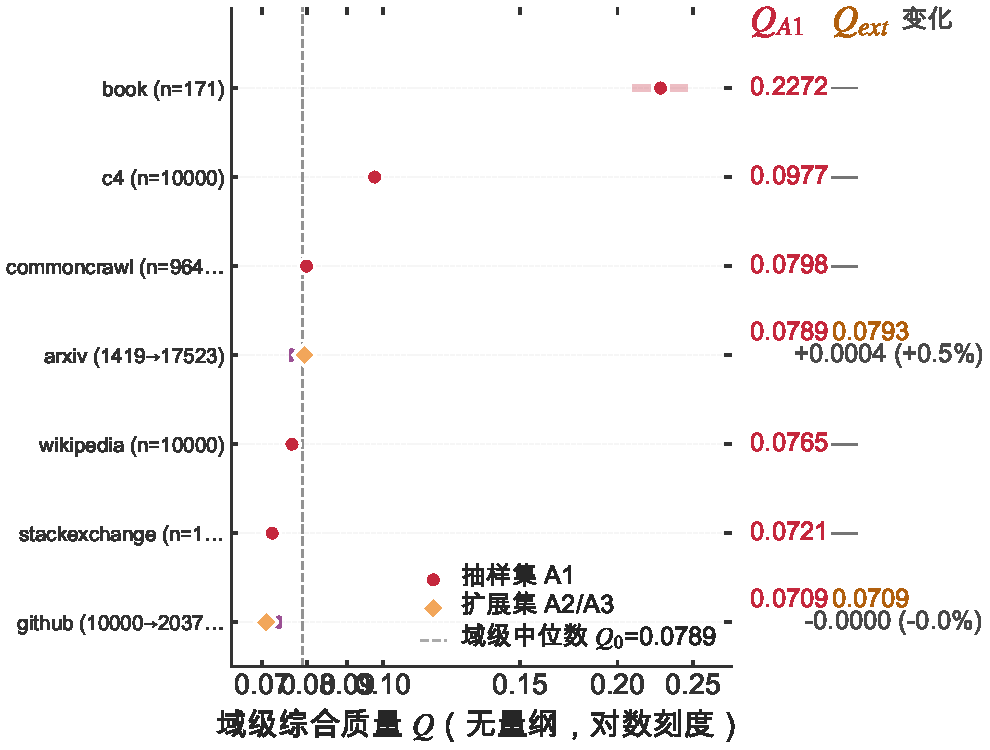
\includegraphics[width=0.9\textwidth,height=0.8\textheight,keepaspectratio]{figures/fig_q1_domain_Q_dumbbell.pdf}
  \caption{抽样集与扩展集域级质量对照}
  \label{fig:q1_domain_Q}
\end{figure}

\begin{figure}[H]
  \centering
  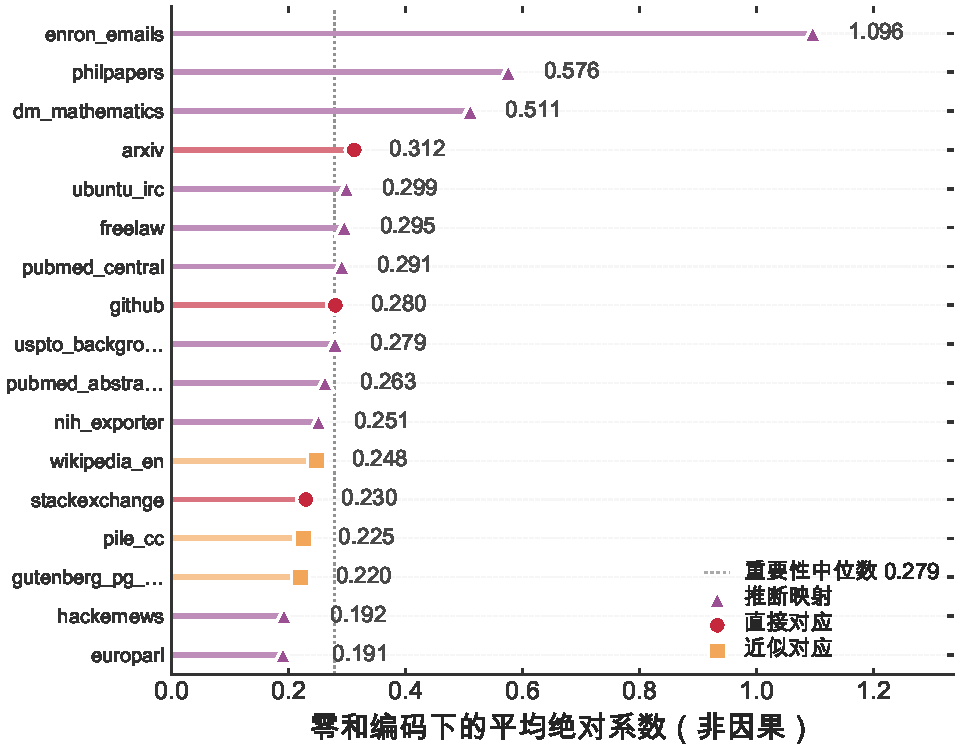
\includegraphics[width=0.9\textwidth,height=0.8\textheight,keepaspectratio]{figures/fig_q1_mixture_importance.pdf}
  \caption{各域配比对损失的重要性排序}
  \label{fig:q1_mixture_imp}
\end{figure}

\begin{figure}[H]
  \centering
  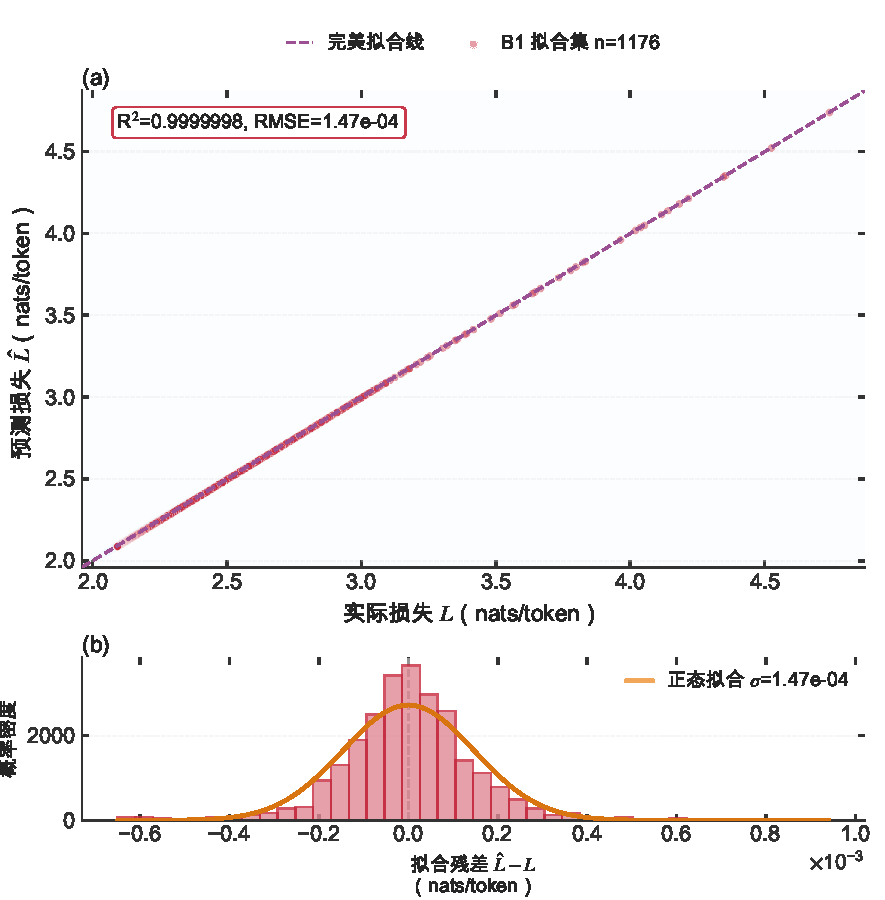
\includegraphics[width=0.8\textwidth,height=0.8\textheight,keepaspectratio]{figures/fig_q2_scaling_fit.pdf}
  \caption{经典标度律拟合优度与残差}
  \label{fig:q2_scaling_fit}
\end{figure}

\begin{figure}[H]
  \centering
  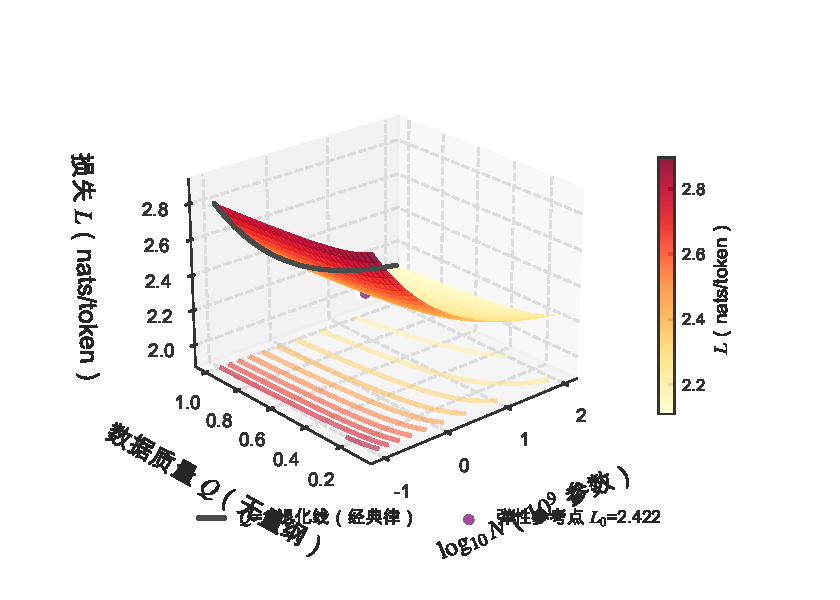
\includegraphics[width=0.9\textwidth,height=0.8\textheight,keepaspectratio]{figures/fig_q2_generalized_surface.pdf}
  \caption{广义标度律损失曲面}
  \label{fig:q2_gen_surface}
\end{figure}

\begin{figure}[H]
  \centering
  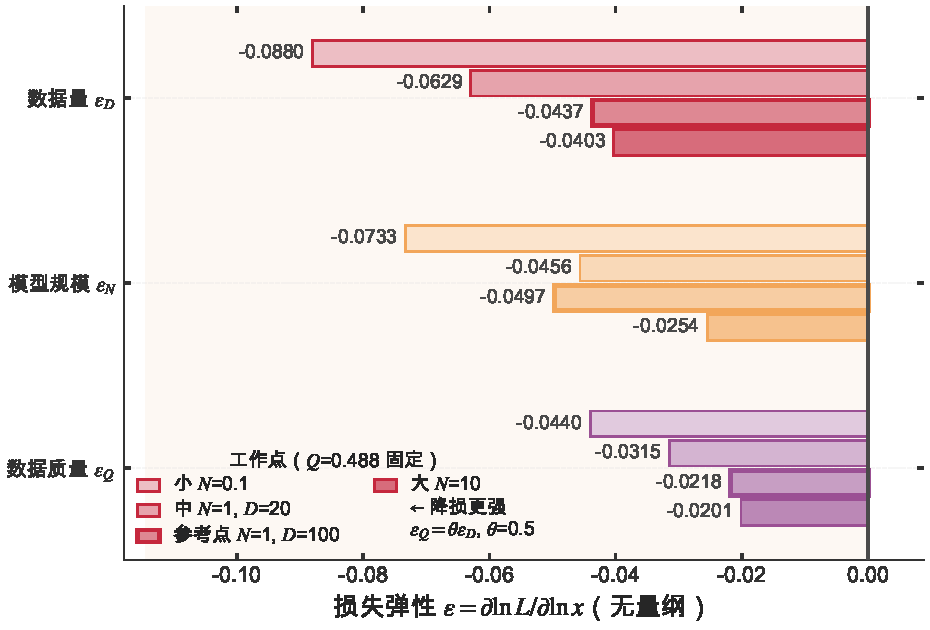
\includegraphics[width=0.9\textwidth,height=0.8\textheight,keepaspectratio]{figures/fig_q2_elasticity_diverging.pdf}
  \caption{各因素损失弹性对照}
  \label{fig:q2_elasticity}
\end{figure}

\begin{figure}[H]
  \centering
  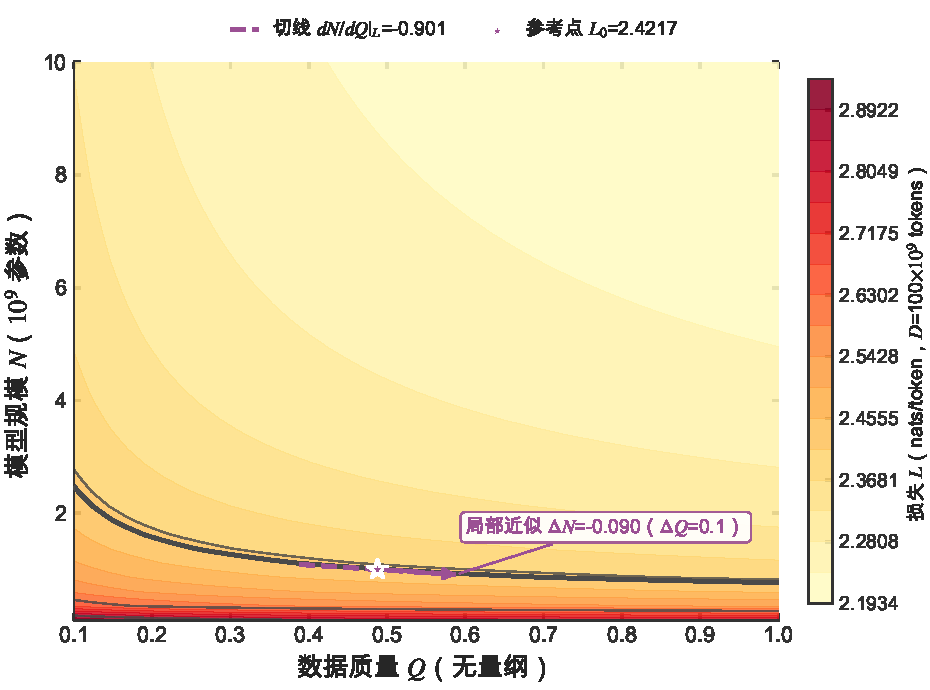
\includegraphics[width=0.9\textwidth,height=0.8\textheight,keepaspectratio]{figures/fig_q2_substitution_contour.pdf}
  \caption{等损失线与质量规模替代}
  \label{fig:q2_substitution}
\end{figure}

\begin{figure}[H]
  \centering
  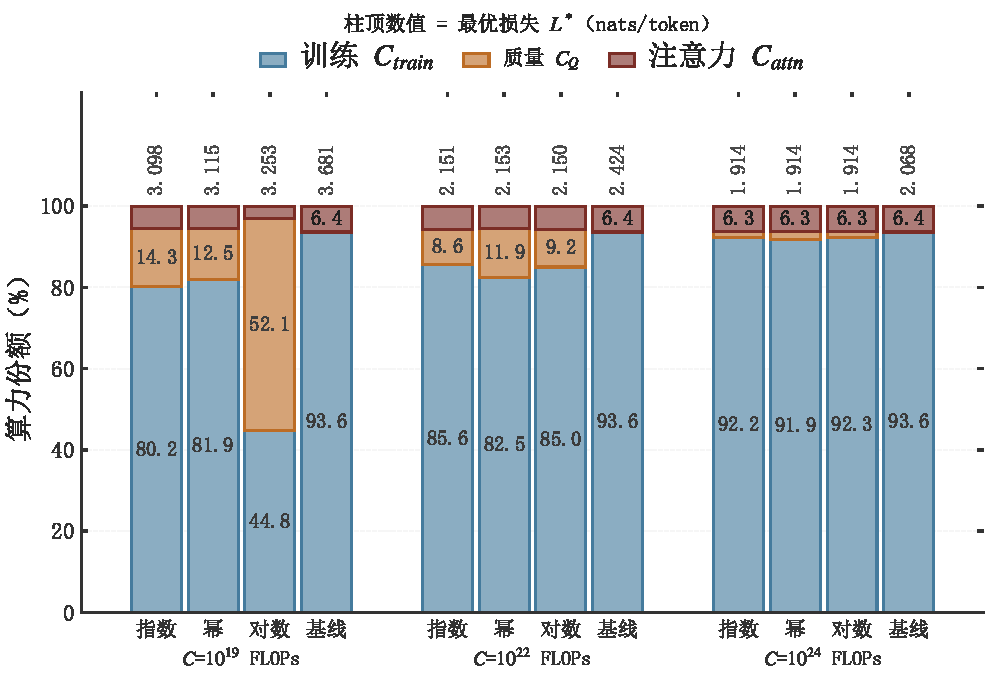
\includegraphics[width=0.9\textwidth,height=0.8\textheight,keepaspectratio]{figures/fig_q3_allocation_stacked.pdf}
  \caption{三档预算下的算力份额构成}
  \label{fig:q3_allocation}
\end{figure}

\begin{figure}[H]
  \centering
  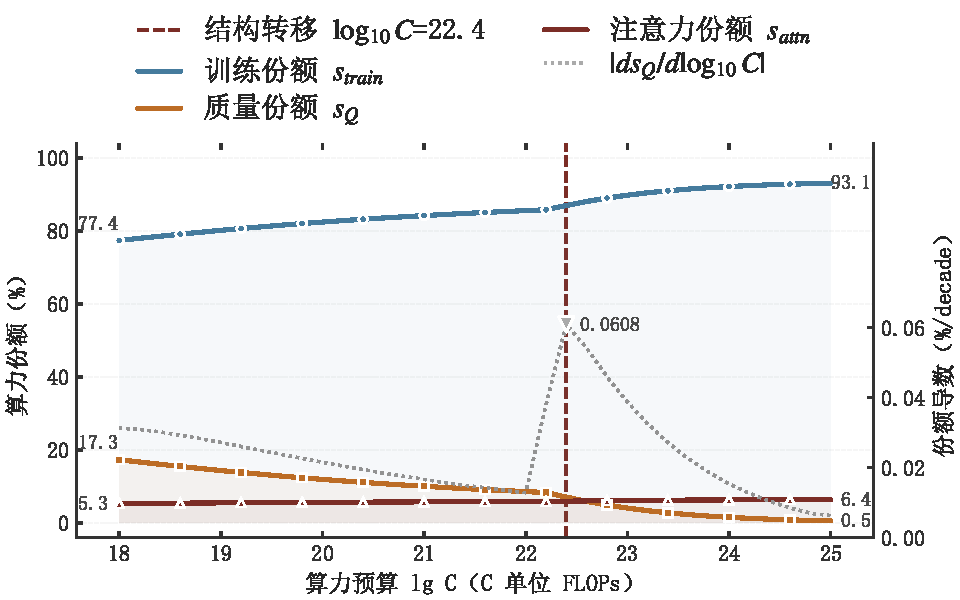
\includegraphics[width=0.9\textwidth,height=0.8\textheight,keepaspectratio]{figures/fig_q3_transition_line.pdf}
  \caption{最优份额演化与结构转移点}
  \label{fig:q3_transition}
\end{figure}

\begin{figure}[H]
  \centering
  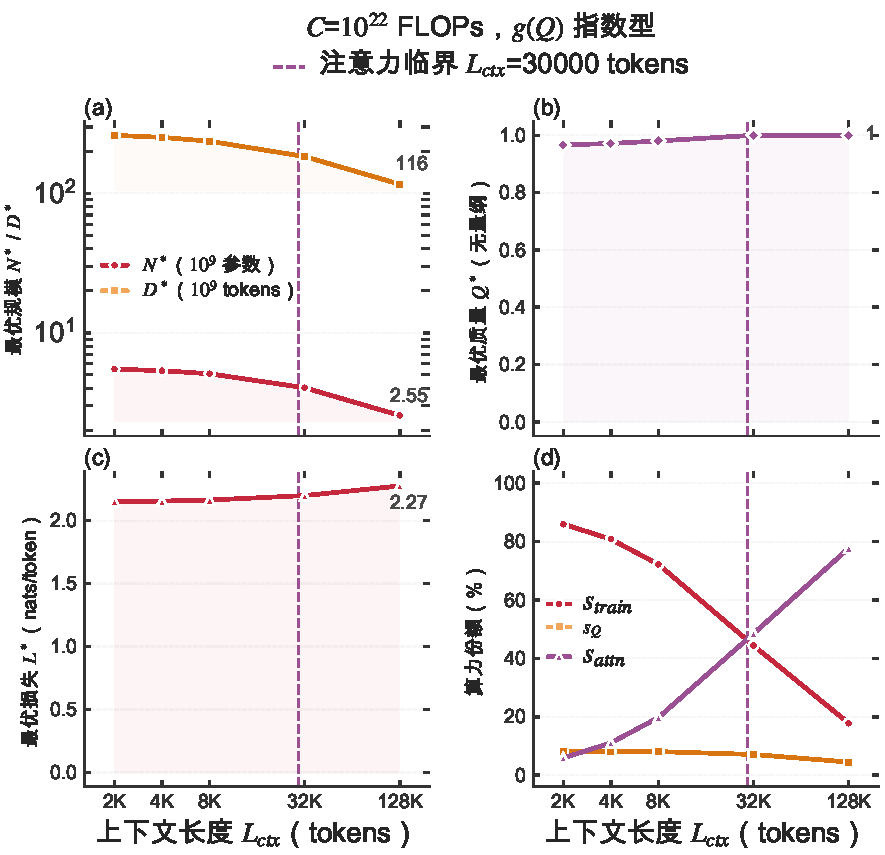
\includegraphics[width=0.8\textwidth,height=0.8\textheight,keepaspectratio]{figures/fig_q3_lctx_panels.pdf}
  \caption{最优配置随上下文长度的变化}
  \label{fig:q3_lctx}
\end{figure}

\begin{figure}[H]
  \centering
  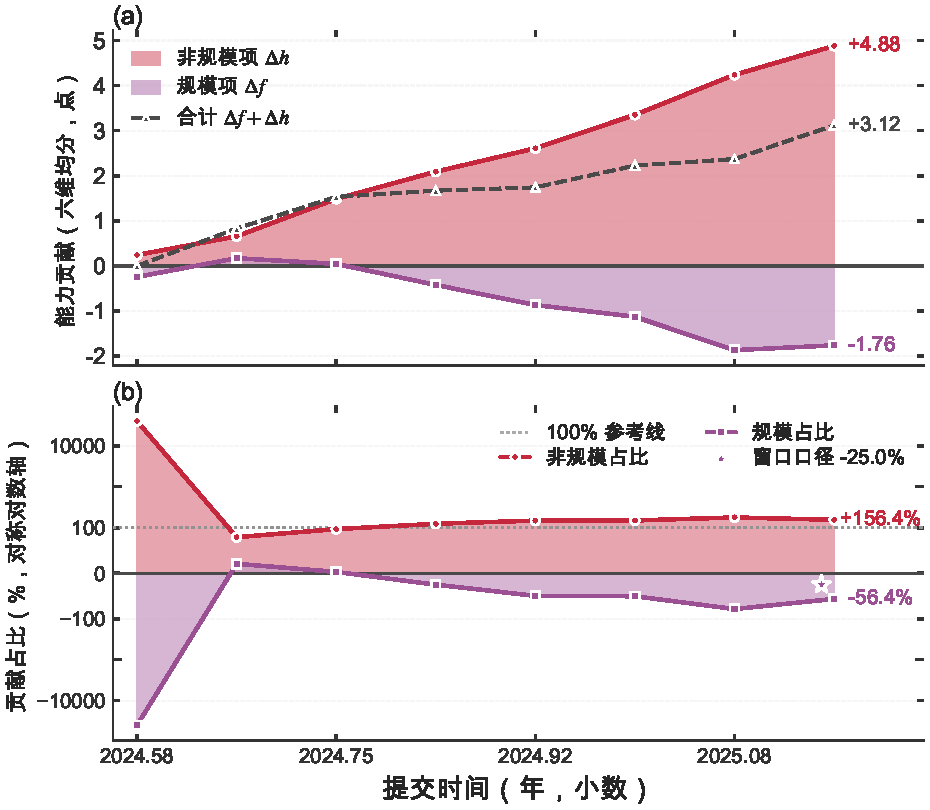
\includegraphics[width=0.8\textwidth,height=0.8\textheight,keepaspectratio]{figures/fig_q4_contribution_decomp.pdf}
  \caption{规模与非规模贡献分解}
  \label{fig:q4_contribution}
\end{figure}

\begin{figure}[H]
  \centering
  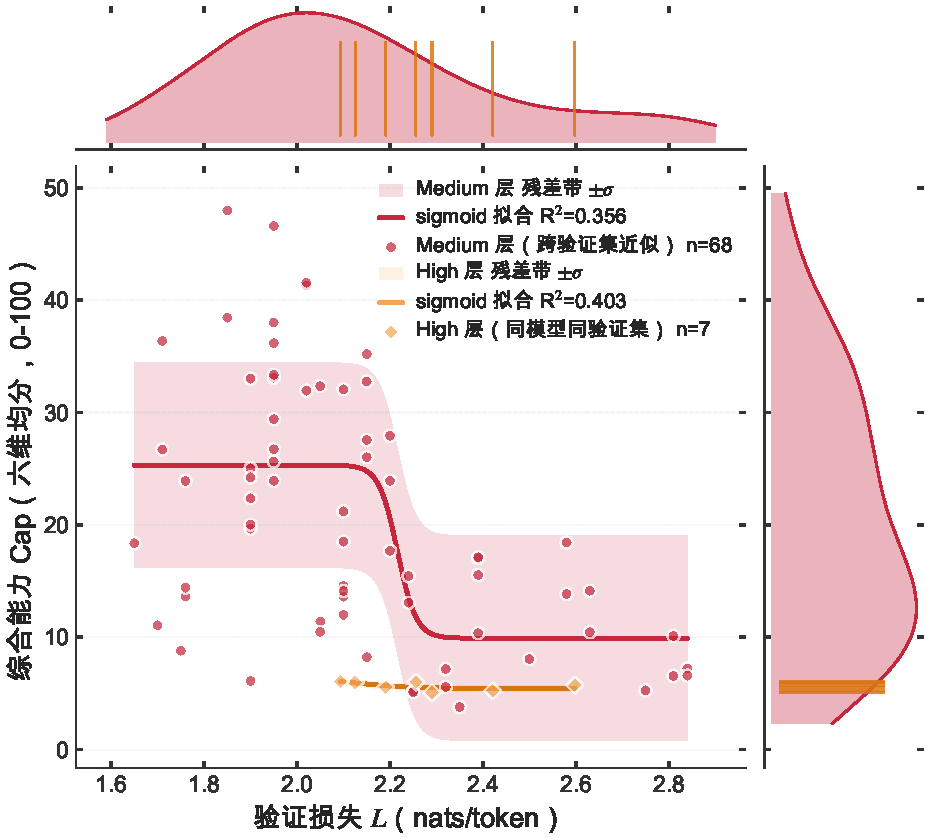
\includegraphics[width=0.8\textwidth,height=0.8\textheight,keepaspectratio]{figures/fig_q4_bridge_scatter.pdf}
  \caption{损失到能力的分层桥接}
  \label{fig:q4_bridge}
\end{figure}

\begin{figure}[H]
  \centering
  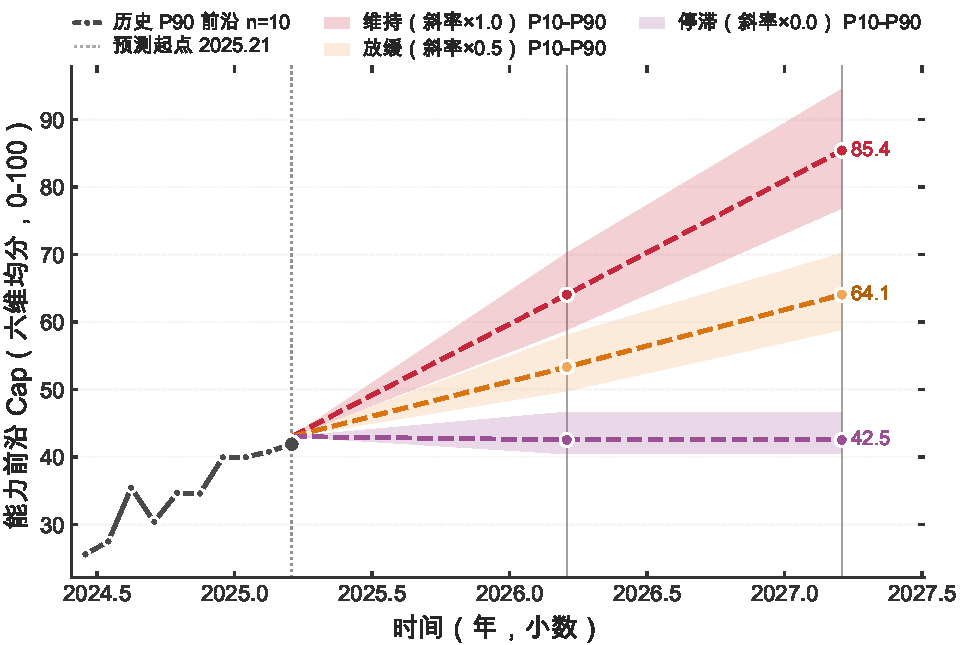
\includegraphics[width=0.9\textwidth,height=0.8\textheight,keepaspectratio]{figures/fig_q4_frontier_fan.pdf}
  \caption{能力前沿情景预测区间}
  \label{fig:q4_frontier}
\end{figure}

\begin{figure}[H]
  \centering
  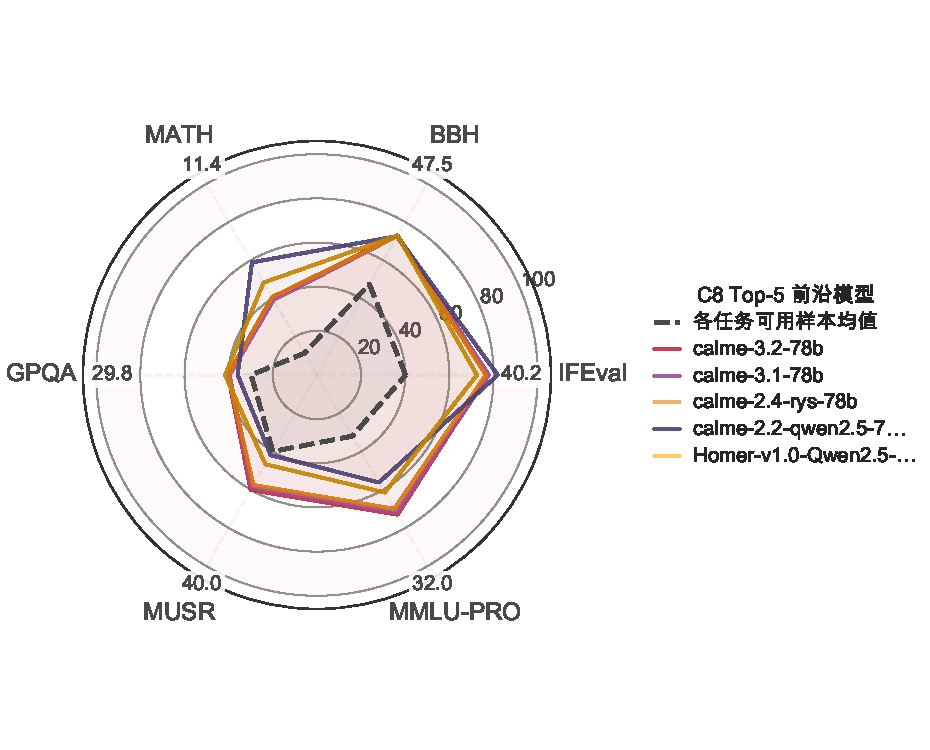
\includegraphics[width=0.8\textwidth,height=0.8\textheight,keepaspectratio]{figures/fig_q4_task_radar.pdf}
  \caption{前沿模型逐任务能力剖面}
  \label{fig:q4_task_radar}
\end{figure}

% === HTML 流程/架构图（paper-figure-html 产出）===
\begin{figure}[H]
  \centering
  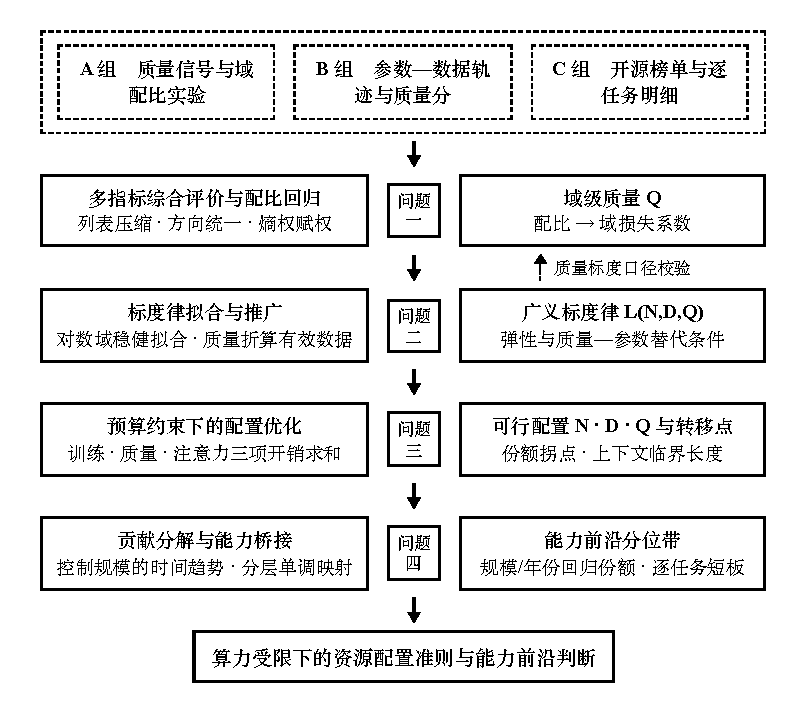
\includegraphics[width=0.88\textwidth,height=0.8\textheight,keepaspectratio]{figures/fig_roadmap.pdf}
  \caption{整体技术路线图}
  \label{fig:roadmap}
\end{figure}

\begin{figure}[H]
  \centering
  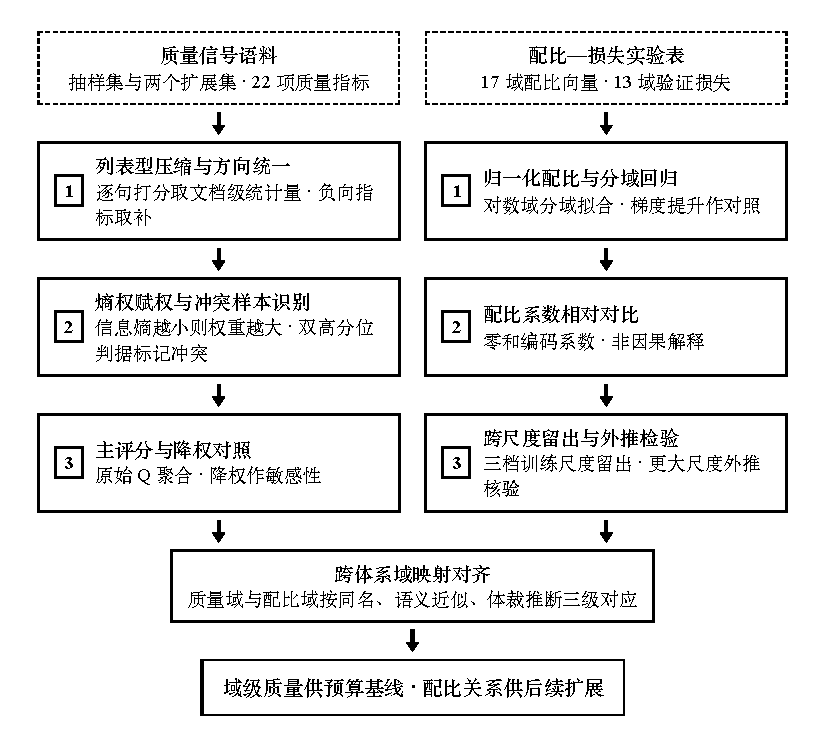
\includegraphics[width=0.9\textwidth,height=0.8\textheight,keepaspectratio]{figures/fig_pipeline_q1.pdf}
  \caption{问题一质量评价数据处理流程}
  \label{fig:pipeline_q1}
\end{figure}

\begin{figure}[H]
  \centering
  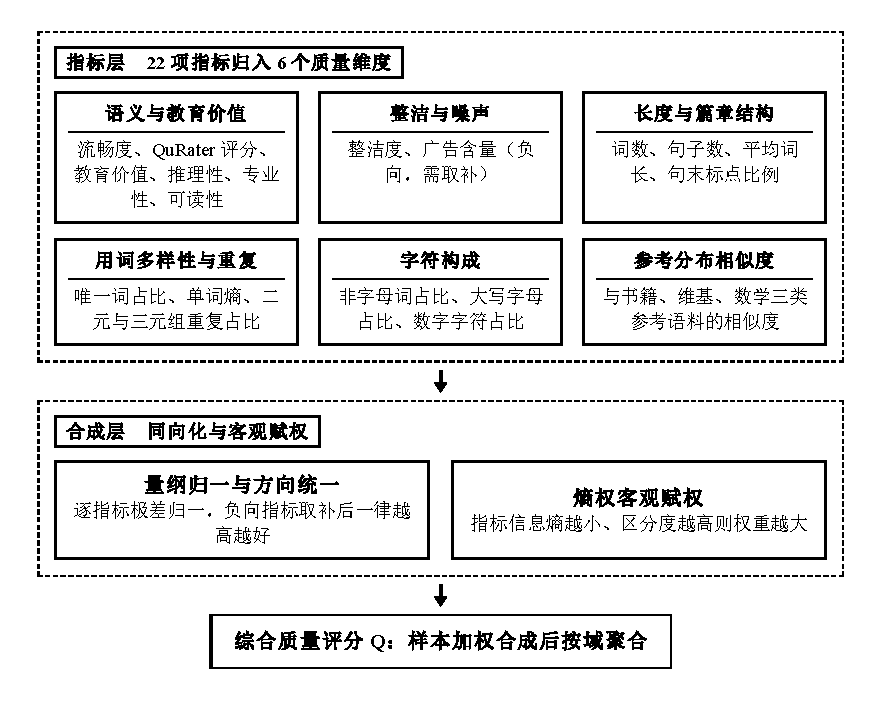
\includegraphics[width=0.9\textwidth,height=0.8\textheight,keepaspectratio]{figures/fig_index_hierarchy.pdf}
  \caption{质量指标体系层次结构}
  \label{fig:index_hierarchy}
\end{figure}

% === TikZ 几何图（算力预算可行域）===
\begin{figure}[H]
  \centering
  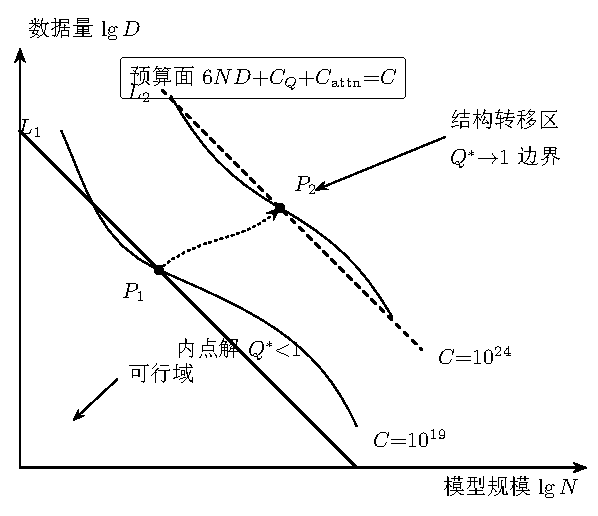
\includegraphics[width=0.8\textwidth,height=0.8\textheight,keepaspectratio]{figures/tikz_q3_feasible.pdf}
  \caption{算力预算可行域与结构转移}
  \label{fig:tikz_q3_feasible}
\end{figure}
